%%%%%%%%%%%%%%%%%%%%%%%%%%%%%%%%%%%%%%%%%%%%%%%%%%%%%%%%%%
%%
%% MARK: Title
%%
%%%%%%%%%%%%%%%%%%%%%%%%%%%%%%%%%%%%%%%%%%%%%%%%%%%%%%%%%%

\chapter*{\S B3. Smooth Function on Periodic Functions}
\setcounter{footnote}{0}

%%%%%%%%%%%%%%%%%%%%%%%%%%%%%%%%%%%%%%%%%%%%%%%%%%%%%%%%%%
%%
%% MARK: Abstract
%%
%%%%%%%%%%%%%%%%%%%%%%%%%%%%%%%%%%%%%%%%%%%%%%%%%%%%%%%%%%

\begin{abstract}
  This exercise%
  \footnote{Joint with P. Donato.}
  gives a simple example of a function on the space of rapidly decreasing sequences that is smooth for the functional diffeology,
  inherited by the smooth periodic functions,
  but not smooth for the ordinary product diffeology.%
\end{abstract}

%%%%%%%%%%%%%%%%%%%%%%%%%%%%%%%%%%%%%%%%%%%%%%%%%%%%%%%%%%
%%
%% MARK: Exercise
%%
%%%%%%%%%%%%%%%%%%%%%%%%%%%%%%%%%%%%%%%%%%%%%%%%%%%%%%%%%%

We consider the subspace $\cE$ of rapidly decreasing complex sequences  $(z_n)_{n\in\ZZ} \in \cE$.
We consider the diffeology ($\clubsuit$) on $\cE$,
inherited by the functional diffeology on the space of
smooth periodic functions,
defined in ``Functional diffeology on Fourier coefficients'' previously.
We denote by $\Can$ the diffeology inherited by the product diffeology,
($\clubsuit$) is finer than $\Can$.

\begin{Article}{Exercise.}{} Show that the linear map $F : \cE \to \CC$,
  $$
    F : (z_n)_{n\in\ZZ} \mapsto \sum_{n\in\ZZ} z_n,
    $$
  is smooth for the diffeology ($\clubsuit$),
  but not for the $\Can$ diffeology.
  
  Hint:
  find a $1$-plot $\gamma : t \mapsto (z_n(t))_{n\in\ZZ}$ for the diffeology $\Can$ such that $F \circ \gamma$ is not smooth.
\end{Article}

\begin{proof}
  We know that the map $j : f \mapsto (f_n)_{n\in\ZZ}$,
  from $\Cinfty_{\rm per}(\RR,\CC)$ to $\cE$,
  where the $f_n$ are the Fourier coefficients of $f$,
  is a diffeomorphism when $\Cinfty_{\rm per}(\RR,\CC)$ is equipped with the functional diffeology and $\cE$ with the diffeology ($\clubsuit$) (op.\,cit.).
  The inverse is given by $j^{-1}: (f_n)_{n\in\ZZ} \mapsto [x \mapsto \sum_{n\in\ZZ} f_n e^{2i\pi n x}]$. Let $\zeta = j^{-1}(z_n)_{n\in\ZZ}$,
  then $F((z_n)_{n\in\ZZ})= \zeta(0)$.
  Therefore $F = \hat 0 \circ j^{-1}$ where $\hat 0$ is the evaluation at the origin,
  $\hat 0(f) = f(0)$.
  Since $\hat 0 : \Cinfty_{\rm per}(\RR,\CC) \to \CC$ is smooth for the functional diffeology and $j^{-1}$ is a diffeomorphism,
  $F$ is smooth.
  
  Next,
  consider the path
  $$
    \gamma : t \mapsto (z_n(t))_{n\in\ZZ} \SpacedText{with} z_n(t) = e^{-\Modulus{n}} e^{i e^{2\Modulus{n}}t},
    $$
  where $t\in\RR$.
  Since every $z_n$ is smooth,
  the path $\gamma$ is smooth with $\cE \subset \prod_{n\in\ZZ}\CC$ equipped with the subset diffeology of the product diffeology.
  Since $\Modulus{z_n(t)} = e^{-\Modulus{n}}$ is rapidly decreasing in $n$,
  the partial sums $\sum_{n=-N}^{N} z_n(t)$ converge for all $t\in \RR$.
  Let $f = F \circ \gamma$,
  that is,
  $$
    f(t) = \sum_{n\in\ZZ} e^{-\Modulus{n}} e^{i e^{2\Modulus{n}}t}.
    $$
  We shall check now that $f$ is not derivable at $t=0$.
  Consider the variation
  \begin{eqnarray*}
    \Delta f(t,0) & = &  {f(t) -f(0) \over t} \\
    &=&  \sum_{n\in\ZZ} { e^{-\Modulus{n}} e^{i e^{2\Modulus{n}}t} - e^{-\Modulus{n}} \over t} \\
    &=& {\sum_{n\in\ZZ}}  {e^{-\Modulus{n}}} \times {e^{i e^{2\Modulus{n}}t} - 1 \over t}. \\
  \end{eqnarray*}
  But,
  $$
    {e^{i e^{2\Modulus{n}}t} - 1 \over t} \xrightarrow[t \to 0]{} i e^{2\Modulus{n}}.
    $$
  Hence,
  $$
    \Delta f(t,0)  \xrightarrow[t \to 0]{} i \sum_{n\in\ZZ} e^{\Modulus{n}},
    $$
  but that is not convergent. Therefore $f$ is not derivable at $t=0$.
\end{proof}

\vfill
\centerline{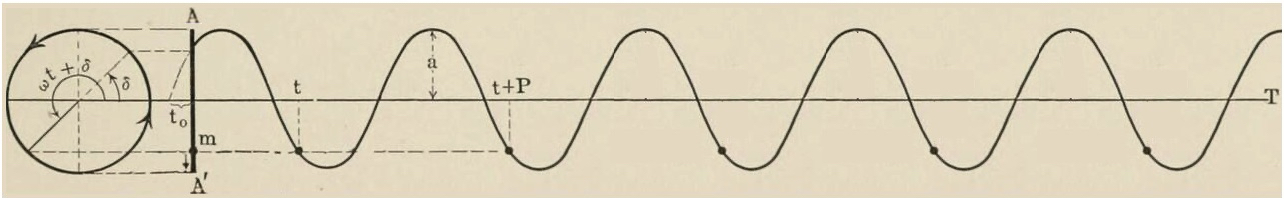
\includegraphics[width=1.0\textwidth]{Figures/Periodic.jpg}}
